\documentclass{beamer}
\usepackage[normalem]{ulem}
\usepackage{graphicx}

\usetheme{metropolis}

%Information to be included in the title page:
\title{Swarm Learning - A Fully Decentralised Approach To Machine Learning}
\author{Josh Pattman}
\institute{University Of Southampton}
\date{March 2023}
\graphicspath{{plots}}

\begin{document}
	\frame{\titlepage}
	
	\section{Why Distributed Machine Learning}
	\begin{frame}
		\frametitle{The Problems}
		\textbf{Privacy}
		\begin{itemize}
			\item Data stored in multiple locations
			\item Cannot share the data between locations for privacy reasons
			\item \emph{Medical records}
		\end{itemize}
		
		\textbf{Performance}
		\begin{itemize}
			\item Machine learning needs lots of processing power
			\item A supercomputer is not available to many
			\item However they may have access to many lower power devices (nodes)
			\item \emph{Company with many unused computers during the night}
		\end{itemize}
	\end{frame}

	\section{Federated Learning}
	\begin{frame}
		\frametitle{Federated Learning - The Current Solution}
		\begin{itemize}
			\item A single model is stored on the server
			\item Server controls many nodes - computers that can perform training
			\item Each node has its own dataset
			\begin{itemize}
				\item This is not shared with other nodes or the server
			\end{itemize}
			\item \textbf{Goal:} Perform machine learning by only sharing the model, not the data
		\end{itemize}
	\end{frame}

	\begin{frame}
		\frametitle{Federated Learning - Variations}
		\begin{itemize}
			\item Many variations of federated learning
			\begin{itemize}
				\item One of the originals is \emph{Federated Averaging (FedAvg)}
				\item Many other algorithms are based off this
			\end{itemize}
		\end{itemize}
	\end{frame}

	\begin{frame}
		\frametitle{Federated Learning - How Does It Work?}
		\begin{itemize}
			\item FedAvg has repeated training steps. Each step:
			\begin{enumerate}
				\item Server sends model to a set of nodes
				\item Nodes perform training on the model
				\item Nodes send their models back to server
				\item New model is the average (mean) of all nodes models
			\end{enumerate}
		\end{itemize}
	\end{frame}

	\begin{frame}
		\frametitle{Federated Learning - Issues}
		\begin{itemize}
			\item Vulnerable to central server going down
			\item Requires that every node has direct access to the server
			\item Few slow nodes slow the whole process down
		\end{itemize}
	\end{frame}

	\section{Swarm Learning}

	\begin{frame}
		\frametitle{Swarm Learning}
		\begin{itemize}
			\item No central server/node
			\item Each node has a distinct model, called the \emph{local model}
			\begin{itemize}
				\item Must keep all local models close to each other
			\end{itemize}
			\item Each node has its own dataset
			\begin{itemize}
				\item This dataset cannot be shared with any other nodes
			\end{itemize}
			\item The goal is to train all local models using all available data
		\end{itemize}
	\end{frame}

	\begin{frame}
		\frametitle{Swarm Learning - How Does It Work?}
		\begin{itemize}
			\item Repeated Training Steps. Each node each step:
			\begin{enumerate}
				\item Perform training on the local model
				\item Send trained model to all neighbours
				\begin{itemize}
					\item This will get saved on the neighbour
				\end{itemize}
				\item New local model is the combination of all neighbours most recent local models
			\end{enumerate}
		\end{itemize}
	\end{frame}

	\begin{frame}
		\frametitle{Swarm Learning - Specifics}
		\begin{itemize}
			\item Different combination methods
			\begin{itemize}
				\item Combine by average
				\item Combine with learning rate
			\end{itemize}
			\item Only combine neighbours who have done more training than this node
			\item Wait for certain number of neighbours to catch up with this node
		\end{itemize}
	\end{frame}

	\begin{frame}
		\frametitle{Swarm Learning vs Issues of Federated Learning}
		\begin{itemize}
			\item \sout{Vulnerable to central server going down}
			\begin{itemize}
				\item No central server - to stop training you would have to take out every node
			\end{itemize}
			\item \sout{Requires that every node has direct access to the server}
			\begin{itemize}
				\item Swarm learning can function on sparse networks of nodes
			\end{itemize}
			\item \sout{Few slow nodes slow the whole process down}
			\begin{itemize}
				\item You never have to wait for a node to communicate, instead use the most recent model it sent
			\end{itemize}
		\end{itemize}
	\end{frame}

	\section{Results}

	\begin{frame}
		\frametitle{Swarm Learning - Performance}
		\begin{itemize}
			\item Following plots are \emph{accuracy} of classifying MNIST Fashion, and x axis is number of epochs trained
			\begin{itemize}
				\item To make the problem a little harder each node only has 10 percent of the dataset
			\end{itemize}
			\item Many different configurations of the algorithm, can drastically affect performance
			\begin{itemize}
				\item In following plots only top 3 configurations sorted by a specific metric
				\item For example metric might be 'area under graph'
			\end{itemize}
		\item Following plots nodes are densely connected
		\end{itemize}
	\end{frame}

	\begin{frame}
		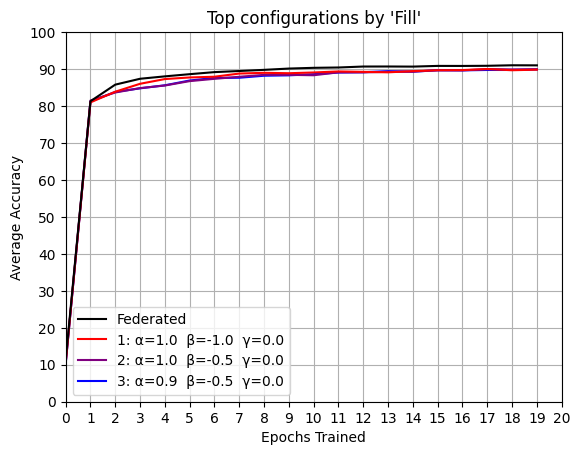
\includegraphics[width = \textwidth]{fill}
	\end{frame}

	\begin{frame}
		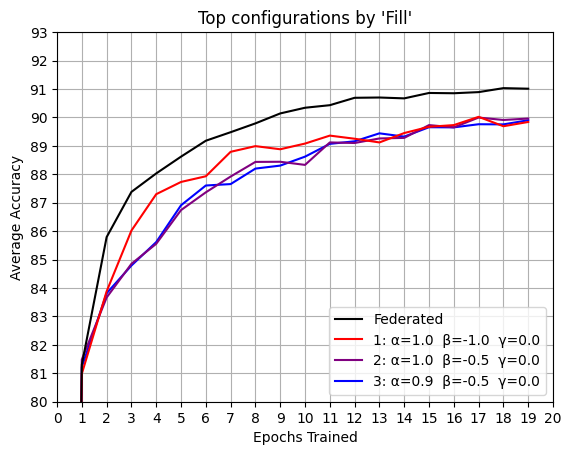
\includegraphics[width = \textwidth]{fill_zoom}
	\end{frame}

	\begin{frame}
		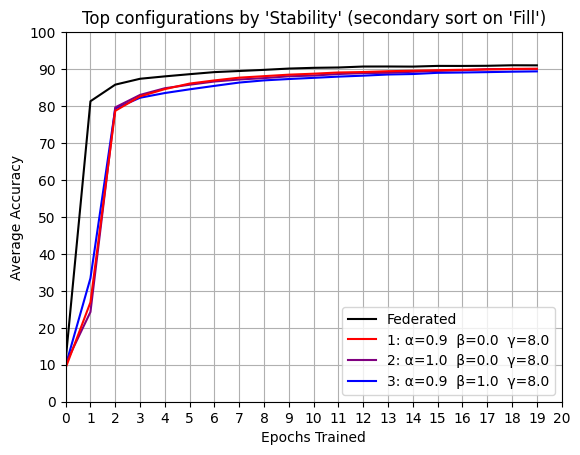
\includegraphics[width = \textwidth]{stability}
	\end{frame}
	
	\begin{frame}
		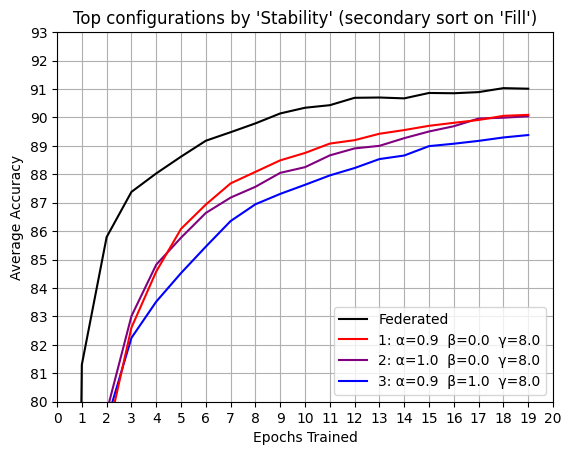
\includegraphics[width = \textwidth]{stability_zoom}
	\end{frame}


	\begin{frame}
		\frametitle{Conclusion}
		\begin{itemize}
			\item Swarm Learning is a promising machine learning algorithm for training a model on data distributed on private data islands
			\item It addresses some of the issues with Federated Averaging, one of the current techniques
			\item It does not perform quite as well as Federated Averaging in a densely connected network
		\end{itemize}
	\end{frame}

	\begin{frame}
		\frametitle{Josh Pattman}
		Thanks for listening!
		\begin{itemize}
			\item LinkedIn: \textbf{linkedin.com/in/josh-pattman}
			\item GitHub: \textbf{github.com/JoshPattman}
		\end{itemize}
	\end{frame}
	
\end{document}